\documentclass{beamer}
\mode<presentation>
\usepackage{amsmath,amssymb,mathtools}
\usepackage{textcomp}
\usepackage{gensymb}
\usepackage{adjustbox}
\usepackage{subcaption}
\usepackage{enumitem}
\usepackage{multicol}
\usepackage{listings}
\usepackage{url}
\usepackage{graphicx}
\def\UrlBreaks{\do/\do-}

\usetheme{Boadilla}
\usecolortheme{lily}
\setbeamertemplate{footline}{
\leavevmode
\hbox{
\begin{beamercolorbox}[wd=\paperwidth,ht=2ex,dp=1ex,right]{author in head/foot}
\insertframenumber{} / \inserttotalframenumber\hspace*{2ex}
\end{beamercolorbox}}
\vskip0pt
}
\setbeamertemplate{navigation symbols}{}

\lstset{
frame=single,
breaklines=true,
columns=fullflexible,
basicstyle=\ttfamily\tiny
}

\numberwithin{equation}{section}

\newcommand{\myvec}[1]{\ensuremath{\begin{pmatrix}#1\end{pmatrix}}}
\let\vec\mathbf

\title{Matgeo Presentation - Problem 4.3.38}
\author{Revanth Siva Kumar.D -- EE25BTECH11048}

\begin{document}

\begin{frame}
\titlepage
\end{frame}

\begin{frame}{Problem Statement}
Find the equation of the line joining the points $(3,1)$ and $(9,3)$. 
\end{frame}

\begin{frame}{Solution:}
\textbf{Solution :} 

Given 
\begin{align}
    \vec{A}=\myvec{3\\1} \vec{B}=\myvec{9\\3} 
    \label{eq:points}
\end{align}
Let us assume line equation to be:
\begin{align}
    \vec{n}^T \vec{x} = c
\end{align} 
    We get the line equation on solving \[\myvec{\vec{A}&\vec{B}}^T\vec{n}=c\myvec{1\\1}\] 

The line passes through the points from \eqref{eq:points} substituting, we get:
\begin{align}
    \myvec{3 & 9 \\
       1 & 3  }^T\vec{n}=c\myvec{1 \\ 1}
\end{align}

\begin{align}
    \myvec{3 & 1 \\
       9 & 3  }\vec{n}=c\myvec{1 \\ 1}
\end{align}
\end{frame}
\begin{frame}{Solution:}
Now by Gaussian Elimination solve:
\begin{align}
\myvec{3 & 1 & \big| & 1 \\
         9 & 3 & \big| & 1 }
\end{align}

\begin{align}
R_{1} &\leftarrow \frac{1}{3}R_{1} \nonumber\\
\Rightarrow\ 
&\myvec{1 & \frac{1}{3} & \big| & \frac{1}{3} \\
         9 & 3 & \big| & 1 }
\end{align}

\begin{align}
R_{2} &\leftarrow R_{2}-9R_{1} \nonumber\\
\Rightarrow\ 
&\myvec{1 & \frac{1}{3} & \big| & \frac{1}{3} \\
         0 & 0 & \big| & -2 }
\end{align}
By the assumption that line equation is $\vec{n}^T\vec{x}=1$ which doesn't pass through origin we are not getting any solution.So our assumption is wrong and origin lies on the line . 
So consider \begin{align}
    \vec{n}^T \vec{x} = 0
\end{align} 
\end{frame}
\begin{frame}{Solution:}
$c=0$ because origin lies on the line and solving:
so now,Assume the line equation:
\[
\vec{n}^T \vec{x} = 0, \quad 
\vec{n} = \myvec{n_1\\n_2}
\]
Line passes through points $\vec{A}$ and $\vec{B}$

\begin{align}
\vec{n}^T \vec{A} = 0 \implies 3 n_1 + 1 n_2 = 0
\end{align}
\begin{align}
    \vec{n}^T \vec{B} = 0 \implies 9 n_1 + 3 n_2 = 0
\end{align}


Matrix form:
\begin{align}
    \myvec{3 & 1 \\ 9 & 3} \myvec{n_1\\n_2} = \myvec{0\\0}
\end{align}

Augmented matrix:
\begin{align}
\myvec{3 & 1 &\big|& 0 \\ 9 & 3 & \big| & 0}
\end{align}
\end{frame}
\begin{frame}{Solution:}
\begin{align}R_{1} &\leftarrow \frac{1}{3}R_{1} \nonumber\\&
\Rightarrow \myvec{1 & \frac{1}{3} & \big| & 0 \\ 9 & 3 & \big| & 0}
\end{align}

\begin{align}R_{2} &\leftarrow R_{2}-9R_{1} \nonumber\\&
\Rightarrow \myvec{1 & \frac{1}{3} & \big| & 0 \\ 0 & 0 & \big| & 0}
\end{align}

From first row:
\begin{align}
n_1 + \frac{1}{3} n_2 = 0 \implies n_1 = -\frac{1}{3} n_2\\
\end{align}
\end{frame}
\begin{frame}{Solution:}
Let,
\begin{align}
n_2 = 3 \implies n_1 = -1\\
\vec{n} = \myvec{-1\\3}
\end{align}

\begin{align}
    \vec{n}^T \vec{x} = 0 \implies \myvec{-1 & 3} \vec{x} = 0 
\end{align}
\textbf{Final Answer}
Required Equation is \begin{align*}
\boxed{\myvec{-1 & 3} \vec{x} = 0}
\end{align*}
\end{frame}

\begin{frame}[fragile]{C Source Code: points.c}
\begin{lstlisting}[language=C]
#include <stdio.h>

// Function to compute normal vector for line through A(3,1) and B(9,3)
void get_normal_vector(double *n1, double *n2) {
    int x1 = 3, y1 = 1;
    int x2 = 9, y2 = 3;

    // Normal vector = [y2-y1, -(x2-x1)]
    *n1 = y2 - y1;    // 3 - 1 = 2
    *n2 = -(x2 - x1); // -(9 - 3) = -6
}

int main() {
    double n1, n2;
    get_normal_vector(&n1, &n2);
    printf("Normal vector: n1=%lf, n2=%lf\n", n1, n2);
    return 0;
}

\end{lstlisting}
\end{frame}

\begin{frame}[fragile]{Python Script: call c.py}
\begin{lstlisting}[language=Python]
import ctypes

# Load C shared library
lib = ctypes.CDLL("./points.so")

# Prepare ctypes doubles
n1 = ctypes.c_double()
n2 = ctypes.c_double()

# Call C function
lib.get_normal_vector(ctypes.byref(n1), ctypes.byref(n2))
print("Normal vector from C:", n1.value, n2.value)

# Save normal vector for plotting
normal_vector = (n1.value, n2.value)

\end{lstlisting}
\end{frame}

\begin{frame}[fragile]{Python Script: plot.py}
\begin{lstlisting}[language=Python]
import numpy as np
import matplotlib.pyplot as plt
import ctypes

# ------------------------
# Load C library to get normal vector
# ------------------------
lib = ctypes.CDLL("./points.so")
n1 = ctypes.c_double()
n2 = ctypes.c_double()
lib.get_normal_vector(ctypes.byref(n1), ctypes.byref(n2))
print("Normal vector from C:", n1.value, n2.value)

# ------------------------
# Points A and B
# ------------------------
A = np.array([3, 1])
B = np.array([9, 3])

# Direction vector along line
D = B - A

# Parameter t for plotting line
t = np.linspace(-1, 2, 100)
line_points = A[:, None] + D[:, None]*t
\end{lstlisting}
\end{frame}
\begin{frame}[fragile]{Python Script: plot.py}
\begin{lstlisting}[language=Python]

# ------------------------
# Plot line and points in 2D
# ------------------------
plt.figure(figsize=(6,6))
plt.plot(line_points[0], line_points[1], color='r', label='Line through A and B')
plt.scatter([A[0], B[0]], [A[1], B[1]], color='b', s=50, label='Points A and B')

# Optional: plot normal vector from origin
origin = np.array([0,0])
plt.quiver(*origin, n1.value, n2.value, angles='xy', scale_units='xy', scale=1,
           color='g', label='Normal vector')

plt.xlabel('X')
plt.ylabel('Y')
plt.title('Line and Normal Vector for Points (3,1) & (9,3)')
plt.grid(True)
plt.axis('equal')
plt.legend()
plt.savefig("line_normal_2d.png")
plt.show()

\end{lstlisting}
\end{frame}

\begin{figure}
     \centering
     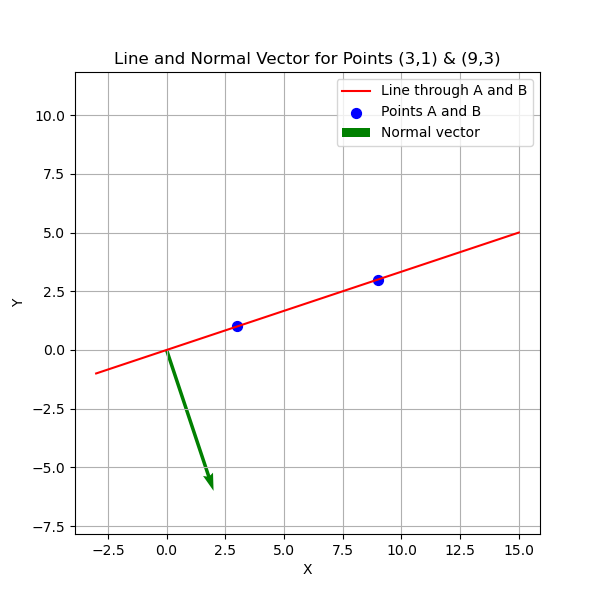
\includegraphics[width=0.7\columnwidth]{figs/Figure_1.png}
     \caption{Plot for the unit vector along PQ}
     \label{fig2}
 \end{figure}

\end{document}
